\documentclass{endm}
\usepackage{endmmacro}
\usepackage{graphicx}
\usepackage{amsthm} % \begin{thm}Here is a new theorem.\end{thm}

\usepackage{amssymb,amsmath,latexsym}
\usepackage[varg]{pxfonts}
%%%%%% ENTER ADDITIONAL PACKAGES
%\usepackage{graphics}
\usepackage{pst-all}
\usepackage{graphicx}
\usepackage{amsmath,amsfonts}
\usepackage{amssymb} % ADDED
\usepackage{times}
\usepackage{latexsym}
\usepackage{fancybox}
\usepackage{algorithm}
%\usepackage{algorithmic}
\usepackage{algorithmicx}
\usepackage{algpseudocode}
\usepackage{setspace}
\usepackage{courier}
\usepackage{verbatim}
\usepackage{hhline}
\usepackage{etex}
\usepackage{graphicx}
\usepackage{listings}
\usepackage{tikz}
\usetikzlibrary{calc,arrows,automata}
\usetikzlibrary{matrix,positioning,arrows,decorations.pathmorphing,shapes}
\usetikzlibrary{shapes,snakes}
\usepackage{graphicx}
%---------------
\usepackage{subfigure}
\usepackage{mathtools}
\usepackage{booktabs}
\usepackage{hyperref}

\lstdefinestyle{mystyle}{
    backgroundcolor=\color{backcolour},   
    commentstyle=\color{codegreen},
    keywordstyle=\color{magenta},
    numberstyle=\tiny\color{codegray},
    stringstyle=\color{codepurple},
    basicstyle=\ttfamily\footnotesize,
    breakatwhitespace=false,         
    breaklines=true,                 
    captionpos=b,                    
    keepspaces=true,                 
    numbers=left,                    
    numbersep=5pt,                  
    showspaces=false,                
    showstringspaces=false,
    showtabs=false,                  
    tabsize=2
}


\tolerance=1
\emergencystretch=\maxdimen
\hyphenpenalty=10000
\hbadness=10000


\floatname{algorithm}{Algorithm}


\def\lastname{Please list your Lastname here}

\begin{document}


\begin{frontmatter}

\title{Métodos Numéricos 2019 - Obligatorio 1}

\author{Bruno Figares (4391788-8),}
\author{Adrián Gioda (4954044-5),}
\author{Daniel Martinez (4462694-5),}
\author{Adriana Soucoff (3190794-8)}

\address{Instituto de Matem\'atica y Estad\'istica\\ Facultad de Ingenier\'ia. Universidad de la Rep\'ublica\\ Montevideo, Uruguay}

\end{frontmatter}


\section{Ejercicio 1}
\subsection{Representación de $f$ en $\mathbb{R}^2$}
%TODO: fix image positioning
\begin{figure}[htbp]
  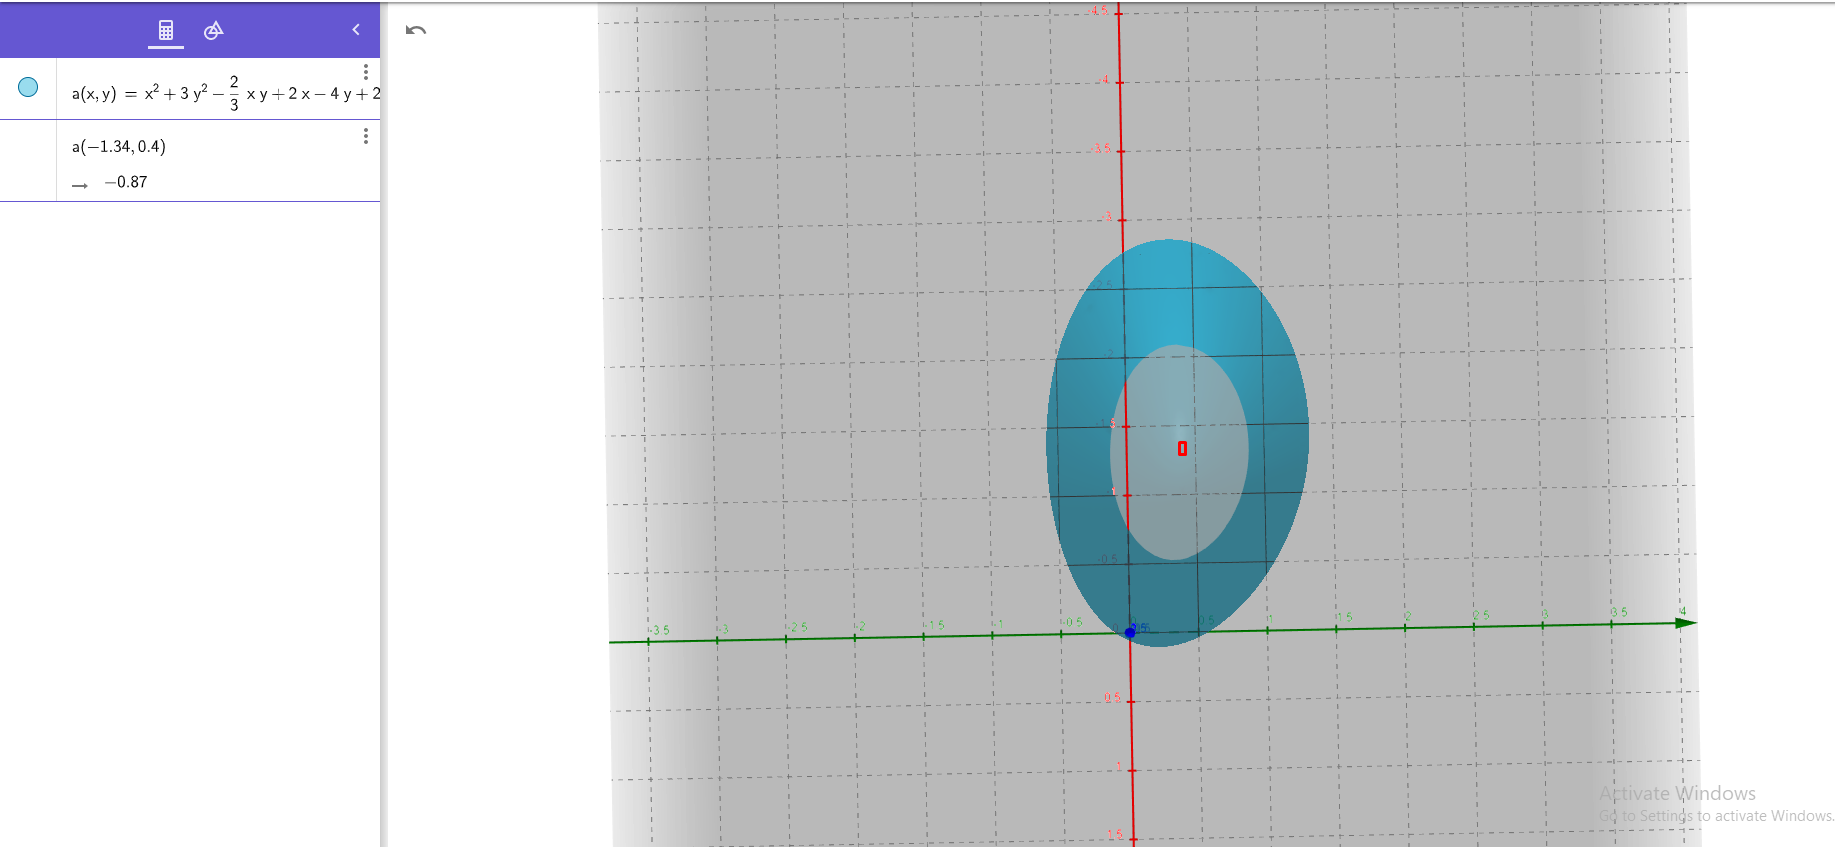
\includegraphics[width=\linewidth]{ej_1_1_1.png}
  \caption{isocurvas de $f(x,y)$}
  \label{fig:1.1.1}
\end{figure}
\begin{figure}[htbp]
  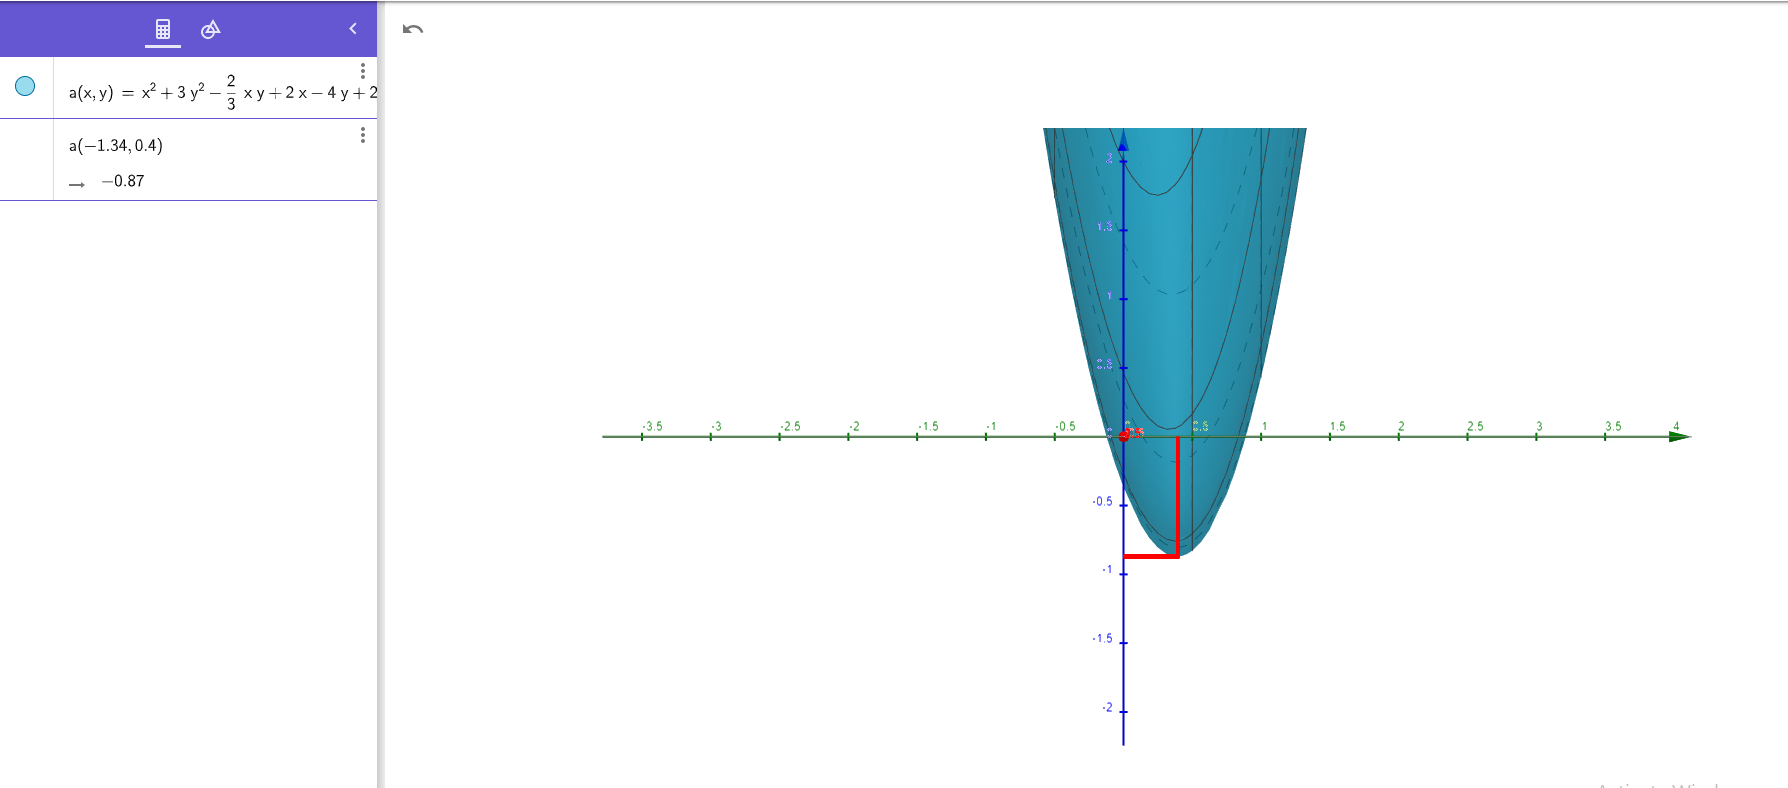
\includegraphics[width=\linewidth]{ej_1_1_2.png}
  \caption{corte transversal de $f(x,y)$}
  \label{fig:1.1.2}
\end{figure}
Se adjuntan dos imágenes  \ref{fig:1.1.1} y \ref{fig:1.1.2}  donde se puede ver la función $f(x,y)$. Su forma parece ser convexa con un mínimo global cerca de cero.
\subsection{Hallar $Q$ y $b$}
$Q \in \mathbb{R}^{2\times2}$ y $b \in \mathbb{R}^{2\times1}$ tienen la siguiente forma

\begin{align}
    Q &= \begin{pmatrix} q_{11} & q_{12} \\ q_{21} & q_{22} \end{pmatrix} & b &= \begin{pmatrix} b_1 \\ b_2 \end{pmatrix}
\end{align}
Sea

\begin{align} 
    f(z) &= (z^{T}Qz - 2b^{T}z) + 2e^{z_x+z_y} \\
    z &= (z_x,z_y)^T \in \mathbb{R}^{2\times1}.
\end{align}
Desarrollando
\begin{equation}
    f(z) = q_{11}z_x^2 + q_{22}z_y^2 + (q_{12} + q_{21})z_x z_y - 2b_1 z_x - 2b_2z_y + 2e^{z_x+z_y}
\end{equation}
Tenemos el siguiente sistema
\begin{equation}
\begin{cases}
q_{11} = 1 \\
q_{12} + q_{21} = -\frac{2}{3} \\
q_{22} = 3 \\
b_1 = -1 \\
b_2 = 2
\end{cases}
\end{equation}

Resolviendolo se tiene que
$Q =  \begin{pmatrix} \phantom{-}1 & -\frac{1}{3} \\ -\frac{1}{3} & \phantom{-}3\end{pmatrix} $
y
$b = \begin{pmatrix} -1\\ 2 \end{pmatrix}$
\subsection{Puntos críticos de $f$}
Podemos ver derivando $\nabla f = 2(Qz -b)+ 2e^{z_x+z_y} = 2*F(z)$, dividiendo entre 2 e igualando a 0 tenemos $ F = 0 $
\subsection{Estimación de puntos críticos}
Se puede ver en las figuras  \ref{fig:1.1.1} y \ref{fig:1.1.2} que aproximadamente se puede obtener el mínimo inspeccionando la gráfica. El mínimo obtenido es $f(-1.34,0.4)= -0.87$
\subsection{Estimando la solución computacionalmente}
Utilizando \lstinline[style=mystyle]{fsolve(@F,[1;1])} tenemos como resultado $(-1.28035, 0.38786)$
\section{Newton Raphson}
\subsection{Descripción de Newton Raphson}
El método de Newton Raphson es un método de aproximación lineal donde miramos la derivada (el jacobiano) en un punto, y buscamos el punto de corte de esta tangente con el 0

El polinomio de taylor de orden 1 en el punto $x^((k))$, con $F$ diferenciable en $x^{(k)}$ es:
\begin{equation*}
F(x) = F(x^{(k)}) + J_F(x^{(k)})(x-x^{(k)})+O(\left \| x-x^{(k)} \right \|^2)
\end{equation*}
truncando el término $O(\left \| x-x^{(k)} \right \|^2)$ y resolviendo $F(x) \approx  0$ tenemos

\begin{equation}
\begin{cases}
 & x^{(k+1)} = x^{(k)} - J_F(x^{(k)})^{-1} F(x^{(k)}) \\
 & x^{(0)}  \in \mathbb{R}^n
\end{cases}
\end{equation}

El determinante de $J_F$ debe ser no nulo para poder invertir la matriz.
El método de Newton rhapson consiste en iterar este proceso, aproximándonos a la solución con cada paso
\subsection{Forma del jacobiano del Ejercicio 1}
Al igual que en la parte 1.3, empezamos por calcular la matriz jacobiana.
    
    Recordamos que la expresion de la funcion F es:
    \begin{equation*}
        F(x,y) = \left( 2x - \frac{2}{3}y + 2 + 2e^{x+y}, 6y - \frac{2}{3}x - 4 + 2e^{x+y} \right)
    \end{equation*}

    Entonces, su jacobiana es:
    \begin{equation}
        \mathbb{J}_F(x,y) =
        \begin{pmatrix}
            \frac{\partial F_1}{\partial x} & \frac{\partial F_1}{\partial y} \\
            \frac{\partial F_2}{\partial x} & \frac{\partial F_2}{\partial y}
        \end{pmatrix}
        =
        \begin{pmatrix}
            \phantom{-}1 + e^{x+y} & -\frac{1}{3} + e^{x+y} \\
            -\frac{1}{3} + e^{x+y} & \phantom{-}3 + e^{x+y}
        \end{pmatrix}
    \end{equation}

    Se quiere probar que $\mathbb{J}_F(x,y) = Q + aa^T$, con $a(x,y) = \begin{pmatrix} 1\\1 \end{pmatrix}\sqrt{e^{x+y}} \in \mathbb{R}^{2 \times 1}$
    es una expresion equivalente.
    
    Desarrollamos la expresion:
    \begin{equation}
        \mathbb{J}_F(x,y) = 
        \begin{pmatrix}
            \phantom{-}1 & -\frac{1}{3} \\
            -\frac{1}{3} & \phantom{-}3
        \end{pmatrix}
        +
        \begin{pmatrix} 1 & 1 \\ 1 & 1 \end{pmatrix} e^{x+y}
        =
        \begin{pmatrix}
            \phantom{-}1 + e^{x+y} & -\frac{1}{3} + e^{x+y} \\
            -\frac{1}{3} + e^{x+y} & \phantom{-}3 + e^{x+y}
        \end{pmatrix}
    \end{equation}
    Se ve entonces que efectivamente se llega a lo mismo.
\subsection{Implementación de Newton Raphson}
Queda implementado en el archivo \lstinline[style=mystyle]{codigo.m}
\subsection{Ejecución de 10 iteraciones de Newton Raphson}
Se implementa en la función \lstinline[style=mystyle]{ej2_3}, el resultado es $(-1.28035, 0.38786)$
\subsection{Comparación con \lstinline[style=mystyle]{fsolve}}
Se implementa en la función  \lstinline[style=mystyle]{ej2_5}, el resultado es $(1.2794*10^{-12},5.1043*10^{-13})$
\subsection{Valor absoluto del error}
\begin{figure}[htbp]
  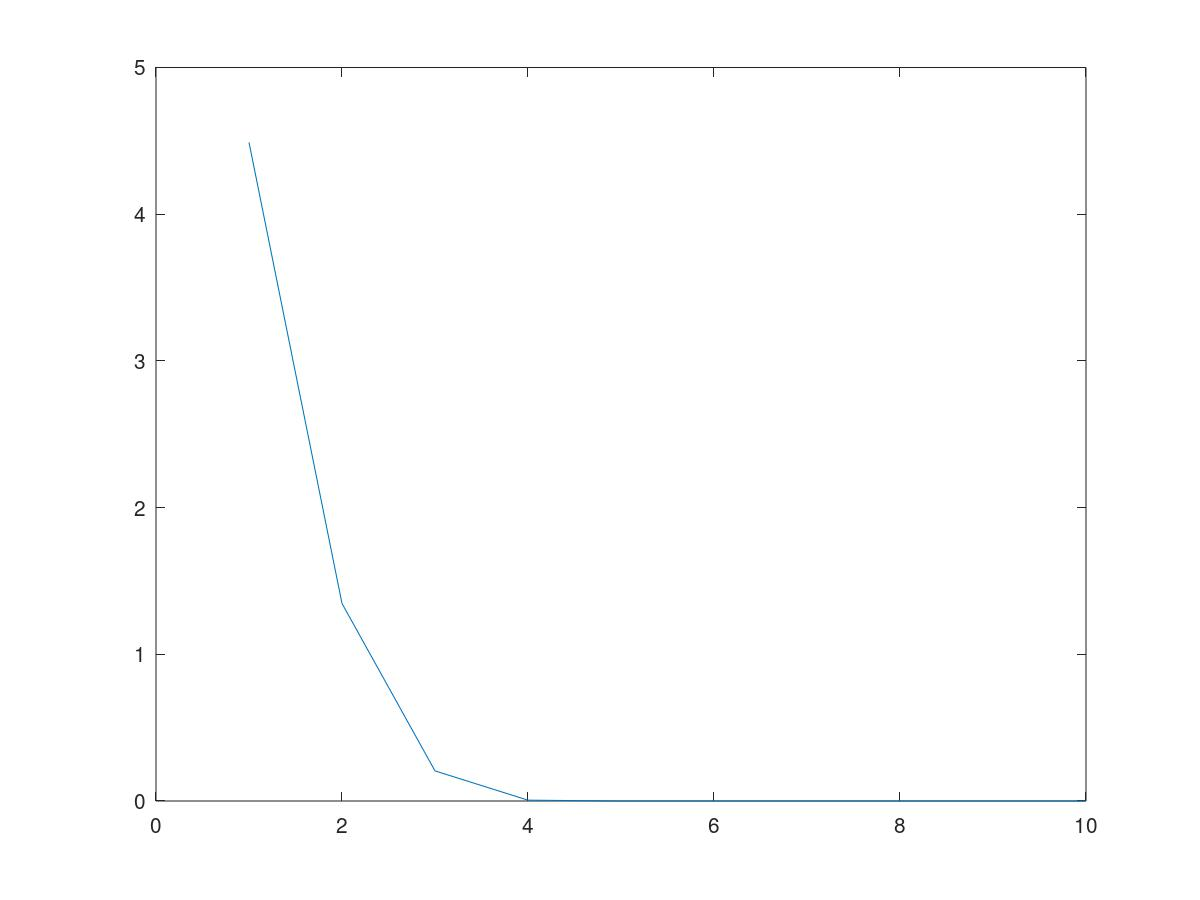
\includegraphics[scale=0.25]{ej_2_6_1.jpg}
  \caption{gráfica lineal de $\| NR(F,iter=x) - fsolve(F) \| $}
  \label{fig:2.6.1}
\end{figure}
\begin{figure}[htbp]
  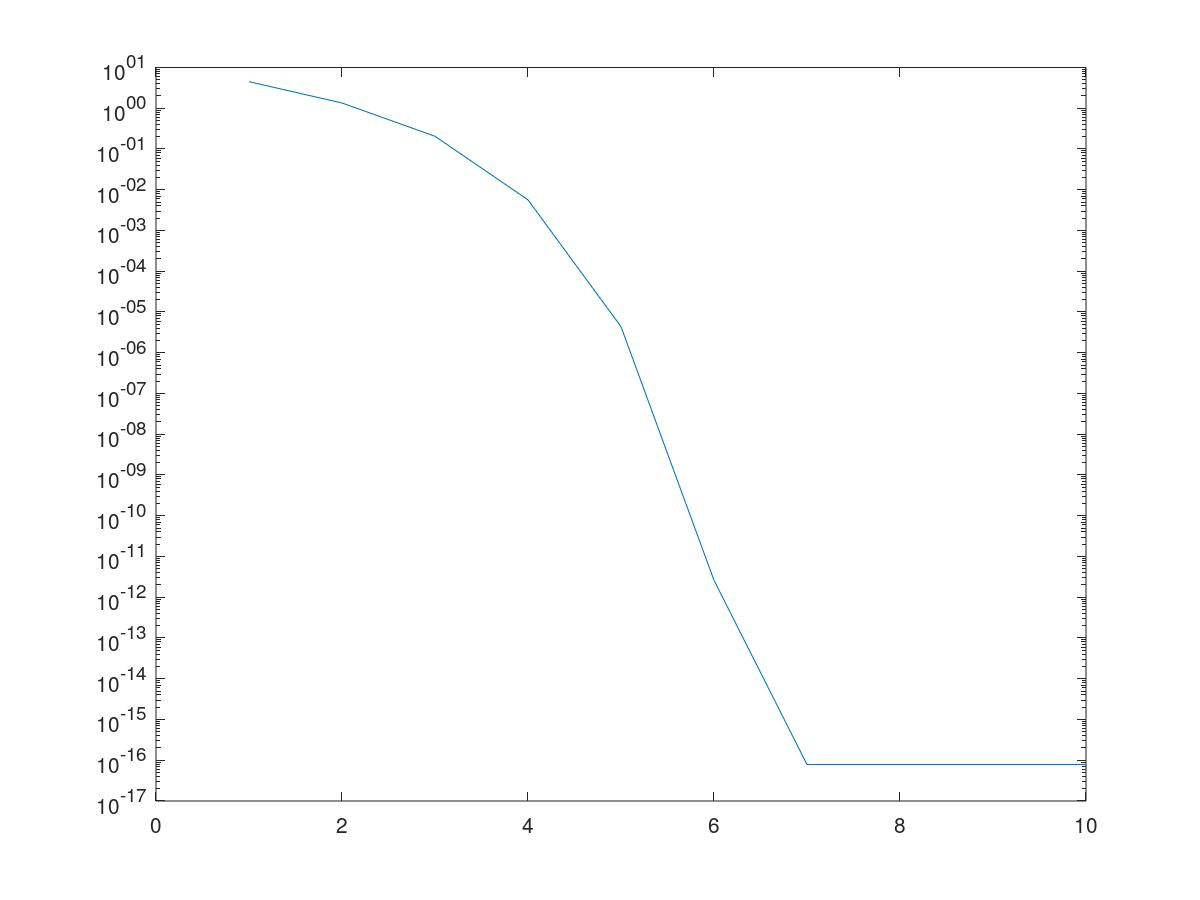
\includegraphics[scale=0.25]{ej_2_6_2.jpg}
  \caption{gráfica logarítmica en $y$ de $\| NR(F,iter=x) - fsolve(F) \| $}
  \label{fig:2.6.2}
\end{figure}
Se implementa en la función  \lstinline[style=mystyle]{ej2_6}. Se presentan dos imágenes, en escala lineal y logarítmica en y en las figuras \ref{fig:2.6.1} y \ref{fig:2.6.2}
\section{Cholesky}
\subsection{Definición}
$Q \in M ^{n\times n} (\mathbb{R})$ una matriz simetrica definida positiva, es decir se cumple:
 $Q=Q^{t}$  y $X^{t}QX > 0 \forall X \neq \vec{0}$
Entonces existe una matriz $C\in M ^{n\times n}$ triangular inferior tal que Q puede ser factorizada como $Q = CC^{t} $
\subsection{Resolución de sistemas por Cholesky}
se quiere resolver el sistema $AX=b$ con $A \in M ^{n\times n} (\mathbb{R})$ una matriz definida positiva
factorizamos $A$ de forma de obtener $A = CC^{t} \Rightarrow CC^{t}X =b$
se hace cambio de variable
\begin{align}
C^{t}X&= Y\\
CY &= b
\end{align}
Se resuelve el sistema triangular (10), C triangular inferior por lo que se usa sustitución hacia adelante:
\begin{align*}
y_{1}&=\frac{b_{1}}{c_{11}}\\
y_{i}&=\frac{1}{c_{ii}}(b_{i}-\sum _{j=1}^{i-1} c_{ij}x_{j}), i=2,...,n
\end{align*}
luego se resuelve el sistema (9) que es triangular superior con sustitución hacia atrás:
\begin{align*}
y_{n}=\frac{b_{n}}{c_{nn}}
y_{i}=\frac{1}{c_{ii}}(b_{i}-\sum _{j=i+1}^{n} c_{ij}x_{j}), i=n-1,...,1
\end{align*}
\subsection{Orden de resolución de sistemas por Cholesky}
El orden de resolver los sistemas anteriores son $n\frac{n+1}{2}$  multiplicaciones, divisiones y el número de sumas  y restas es n $\frac{n-1}{2}$
para resolver el sistema se usa $\mathcal{O}\left(n^{2}\right)$ flops
Para factorizar $A$ como $CC^{t}$ , se hace cambio de variable $L=C^{t}$ y $L^{t}=C$ de esta forma buscamos $A= L^{t}L$   utilizando descomposición QR se obtiene la factorización, el orden de la misma es de $\frac{1}{3}n^{3}$
por lo tanto el orden total es $\frac{1}{3}n^{3} + 2n^{2} \approx \frac{1}{3}n^{3}$
\subsection{Órden de Newton Raphson con Cholesky}
el algoritmo Newton Raphson tiene k iteraciones en cada una se resuelve el sistema lineal con Cholesky que es de orden $\frac{1}{3}n^{3}$  por lo tanto el orden de NR utilizando Cholesky es de  $\frac{k}{3}n^{3}$
\section{Mínimo de una función en $\mathbb{R}^n$}
%Ej4.1
\subsection{Teorema de Gershgorin}
Se busca probar que la matriz Q es siempre definida positiva usando el Teorema de Gershgorin.
Dado $Q \in \mathbb{R}^{n \times n}$, se considera el Teorema aplicado a los numeros reales.
Dadas $q_{ij}$ entradas de Q, sea $R_i = \sum_{i \neq j}\left | q_{ij} \right |$ y sea $D(q_{ij},R_i)$
un entorno cerrado $ [q_{ii}-R_i, q_{ii}+R_i]$, el teorema dice:
\begin{thm}[Teorema de Gershgorin]
    Todo valor propio de Q esta en al menos uno de los entornos cerrados.
\end{thm}
Por otro lado, $Q$ es definida positiva sii $\lambda_i > 0$ $\forall \lambda_i$ valor propio de $Q$
Entonces, basta probar que todos los elementos de los entornos cerrados de Q contienen solo valores positivos.
Especificamente, si $\forall i:$ $1 \leq i \leq n$, $q_{ii} - R_i >0$ entonces $Q$ sera definida positiva.
Generalizando:
Los elementos de $Q$ son:
\begin{equation}
    \begin{cases}
        q_{i,i+1} = \frac{(-1)^i}{3i} \phantom{-} \forall i = 1,...,n-1 \\
        q_{i,i} = 2i-1 \phantom{-} \forall i = 1,...,n
    \end{cases}
\end{equation}
Los radios del intervalo son:
con $n > 1$
\begin{equation}
    \begin{cases}
        R_1 = \frac{1}{3} \\
        R_n = \frac{1}{3(n-1)} \\
        R_i = \frac{1}{3(i-1)} + \frac{1}{3i} \text{ para }  1<i<n
    \end{cases}
\end{equation}
Entonces, para $n > 1$,
\begin{equation}
    \begin{cases}
        q_{i,i} - R_1 = 1 - \frac{1}{3} = \frac{2}{3} > 0 \\
        q_{n,n} - R_n =  2n-1 - \frac{1}{3(n-1)} = \frac{1}{3(n-1)}(6n^2 - 9n + 2) > 0 \phantom{-}\forall n>1 \\
        q_{i,i} - R_i = 2i-1 - \frac{1}{3(i-1)} - \frac{1}{3i} > 0 \phantom{-}\forall n>1
    \end{cases}
\end{equation}
Se prueba entonces que todos los valores propios de $Q$ son positivos y por tanto es una matriz definida positiva.
%Ej4.2
\subsection{Actualización de rango uno de Q}
Se utiliza Referencia dada en la letra del Obligatorio:  Walder,  C.  (2010).  RankkCholesky  Up/Down-dating  on  the  GPU:  gpucholmodV0.  2.arXiv preprint arXiv:1011.1173.


El algoritmo recorre la matriz $L^{t}$  siendo L matriz de factorización de Cholesky de Q
y  la va modificando transformandola en la matriz $\bar{L}^{t}$ siendo $\bar{L}$ matriz de factorización de Cholesky de $Q_{a}$.
Se recorre en un loop inicial por filas de $L^{t}$ , se calcula el elemento de la diagonal de la fila y luego se realiza un loop por las columnas, se calcula en cada elemento el valor dada una fórmula que contiene elementos de la corrida actual y la anterior(la fila anterior).
Se utilizan las variables s y c para almacenar datos de la corrida anterior que serán usados en el cácluo de la siguiente.


$Q=\begin{pmatrix}
l_{11}                &\sqrt{l_{11}}l_{21}   &...                                &... \\ 
\sqrt{l_{11}}l_{21}   &l_{21}^{2}+l_{22}^{2} &...                                &... \\ 
...                   &...                   &l_{31}^{2}+l_{32}^{2}+l_{33}       &... \\
... \\ 
 ...                   &...                   &...                               &l_{n1}^{2}+l_{n2}^{2}+...+l_{nn-1}^{2}+l_{nn} 
\end{pmatrix}$


$aa^{t}=\begin{pmatrix}
a_{1}^{2}         &a_{1}a_{2}     &...  &a_{1}a_{n} \\ 
a_{2}a_{1}        &a_{2}^{2}      &...       &... \\ 
 ...                  &...       &...       &... \\

 ...                   &...       &...       &a_{n}^{2} 
\end{pmatrix}$

$Q_{a}=Q + aa^{t} = \bar{L}\bar{L}^{t}$

se busca obtener $\bar{L}^{t}=\begin{pmatrix}
\sqrt{ \bar{l}_{11}}          &0     &...  &0 \\ 
\bar{l}_{21}       &\sqrt{ \bar{l}_{22}}       &...       &0 \\ 
\bar{l}_{31}                   &...       &...       &0 \\

\bar{l}_{n1}                   &...       &...       &\sqrt{ \bar{l}_{nn}}
\end{pmatrix}$


$\sqrt{ \bar{l}_{11}} =\sqrt{ (\sqrt{{l}_{11})}^{2} +a_{1}^{2}}$


$\bar{l}_{21} =  \frac{\sqrt{{l}_{11}}{l}_{21} +a_{2}a_{1}}{\sqrt{(\sqrt{{l}_{11}})^{^{2}}+a_{1}^{2}}}$


tenemos elementos de la corrida de la fila 1 y elementos de la corrida de la fila 2 en la que se esta, factorizan esta cuenta de froma de independizar los elementos de la corrida anterior con c y s 
para este caso:

$c_{1}=\frac{\sqrt{ (\sqrt{{l}_{11})}^{2} +a_{1}^{2}}}{\sqrt{{l}_{11}}}$


$s_{1}=\frac{a_{1}}{{l}_{11}}$


son utilizados en el cálculo de los elementos que no son de la diagonal
según la fórmula: $\bar{l}_{ij} =  \frac{{{l}_{ij}} +{s}_{i}a_{j}}{c_{i}}$
%Ej4.3
\subsection{Thomas}
%Ej4.4
\subsection{NR incorporando Cholesky, NR2}
(ver codigo)
%Ej4.5
\subsection{Orden NR2}
El orden de NR2 es dado por k iteraciones de NR y en cada una de las iteraciones se calcula: la actualización de rango uno de Q (  orden $n^{2}$ ) , la descomposición de Cholesky ultilizando método de Thomas (orden n), y sustitución hacia atrás (  orden $n^{2}$ ) por lo tanto el orden de NR2 es $kn^{2}$. 

%Ej5
\section{Pruebas Experimentales}
Quinto problema
%Ej5.1
\subsection{}
%Ej5.2
\subsection{Verificación de $z^{NR}$}
En la tabla \ref{tab:table_5_2} se muestra la norma de $F(z)$ para distintos valores de dimension $n$.
\begin{table}[h!]
    \begin{center}
      \caption{Your first table.}
      \label{tab:table1}
      \begin{tabular}{l|c|r} % <-- Alignments: 1st column left, 2nd middle and 3rd right, with vertical lines in between
        \textbf{n} & \textbf{$||F(z^{NR})||$}\\
        \hline
         100 & 3.574573332905249e-014\\
         200 & 1.175361818307876e-013\\
         300 & 1.997171185243193e-013\\
         400 & 3.256674181109525e-013\\
         500 & 4.902233609479727e-013\\
        1000 & 1.403048923326327e-012\\
        2000 & 3.877314569665418e-012\\
        3000 & 7.960022321886946e-012\\
        4000 & 1.081169278301875e-011\\
        5000 & 1.555144859221123e-011\\
        \hline
      \end{tabular}
    \end{center}
  \end{table}  
Se puede ver que para todos los tamaños, se llega casi a anular la función en 20 iteraciones.
%Ej5.3
\subsection{Tiempo de ejecución de NR2}
Con el fin de estudiar el tiempo de ejecución del algoritmo de NR2, se lo aplica para distintos valores de dimension $n$.
\begin{equation*}
    n = [1, 2, 3, 4, 5, 10, 20, 30, 40, 50] \times 100
\end{equation*}
A continuación se muestran los resultados:
\begin{figure}[h!]
    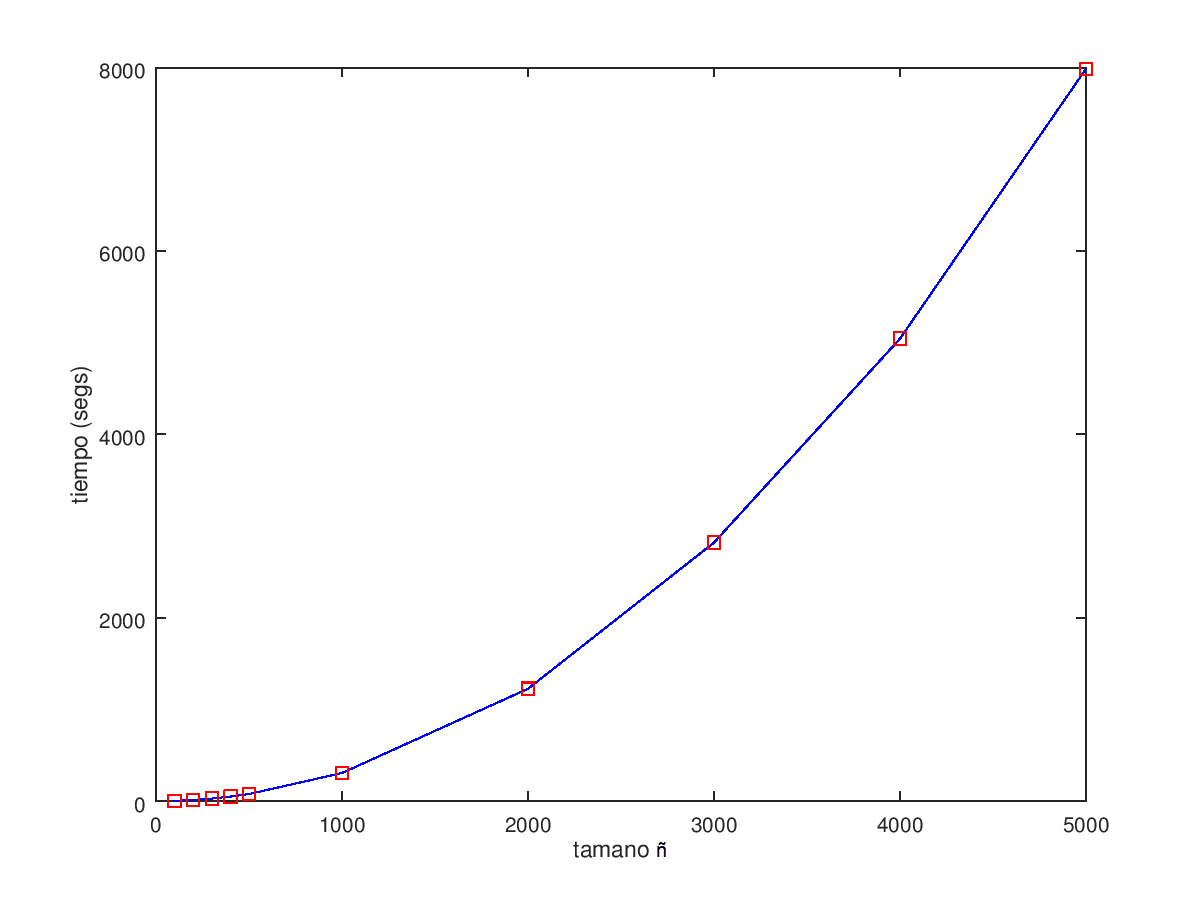
\includegraphics[width=\linewidth]{Grafica_5_3_1.png}
    \caption{Tiempo de ejecución del algoritmo NR2.}
    \label{fig:Grafica_5_3_1}
\end{figure}
\begin{figure}[h!]
    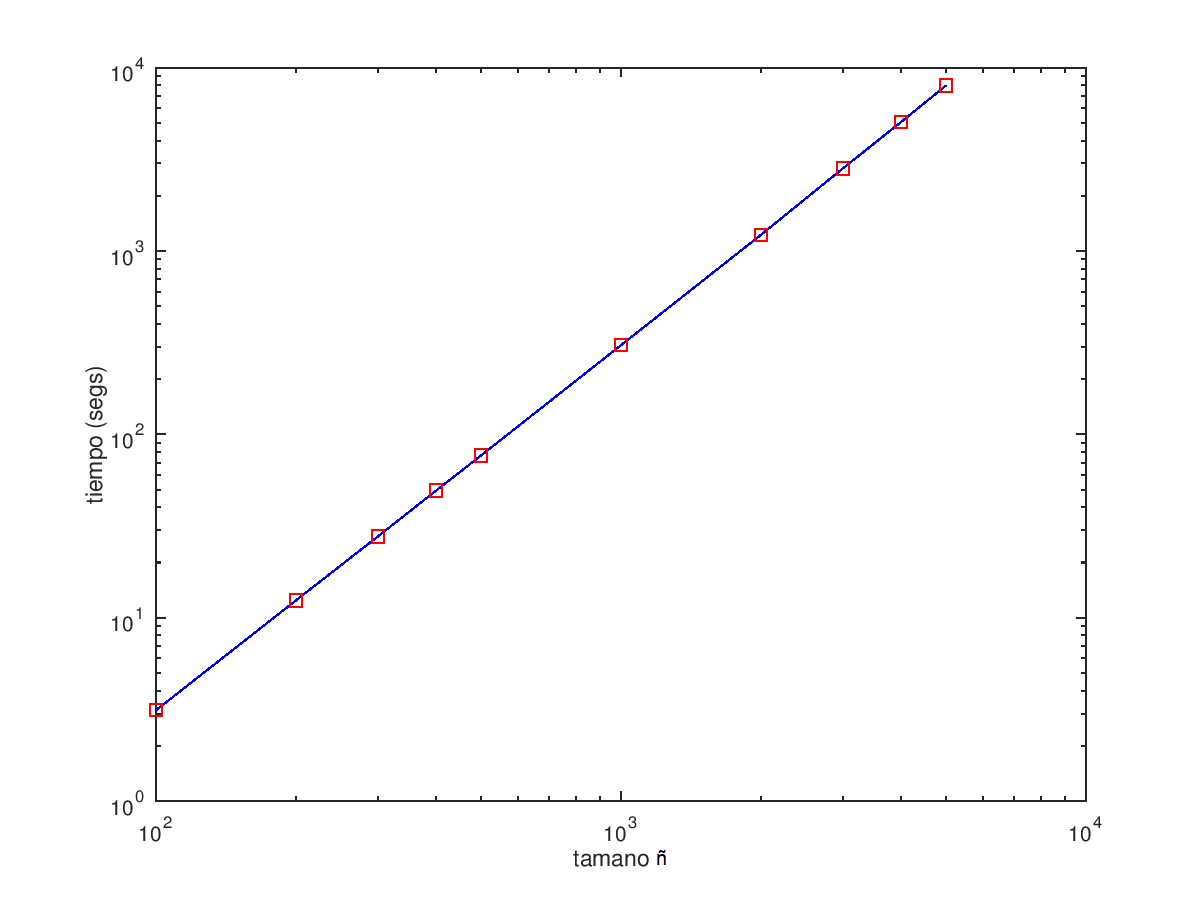
\includegraphics[width=\linewidth]{Grafica_5_3_2.png}
    \caption{Tiempo de ejecución del algoritmo NR2 en escala logaritmica.}
    \label{fig:Grafica_5_3_2}
\end{figure}
En la figura \ref{fig:Grafica_5_3_2}, se puede ver un comportamiento lineal de los datos.
Esto concuerda con lo visto en la sección 4.5, donde se vio que el tiempo de ejecucion es $O(n^2)$.
Comprobemoslo:
\begin{align}
    T(n) &= kn^2 \\
    log(kn^2) &= log(k) + 2log(n) \\
    \text{ C.V.}& \rightarrow y = log(kn^2) \text{ ; } x = log(n) \\
    y &= a + bx
\end{align}
%Ej5.4
\subsection{Ajuste polinomial del tiempo de ejecución}
Utilizando la funcion polyfit de Octave, se ajustan los datos de la sección 5.3 con un polinomio de grado 2.
\begin{figure}[h!]
    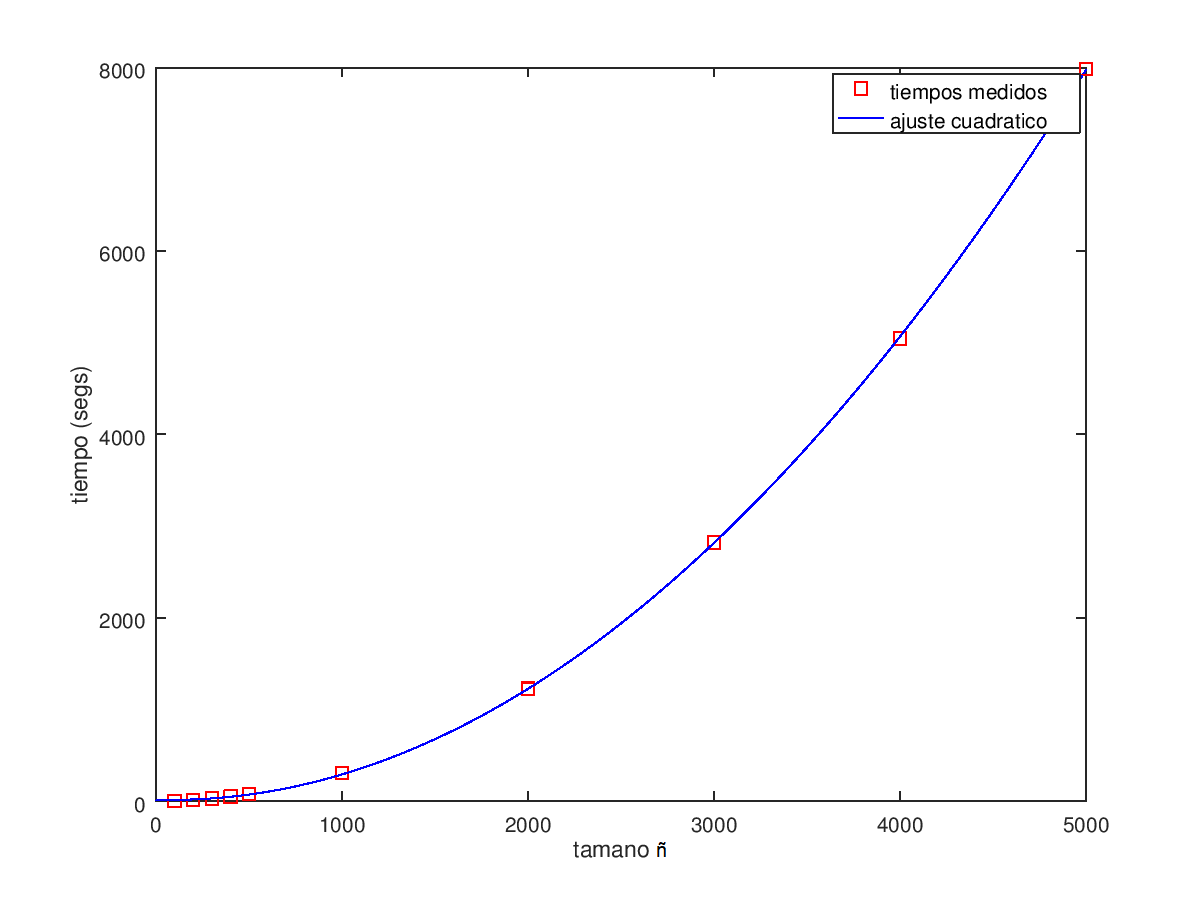
\includegraphics[width=\linewidth]{Grafica_5_4.png}
    \caption{Ajuste cuadratico del tiempo de ejecucion de NR2.}
    \label{fig:Grafica_5_4}
\end{figure}
Como se ve en la figura, con un polinomio de grado 2 se logran ajustar correctamente los datos.
\clearpage
\end{document}\grid
